\documentclass[letterpaper]{article}
\usepackage[spanish,es-tabla]{babel}
\usepackage{indentfirst}
\usepackage{float}
\usepackage[utf8]{inputenc}
\usepackage{graphicx}

\begin{document}
    \subsection*{DTF con zero-padding}
Se realizo ahora nuevamente el calculo de la DFT de las señales de la seccion anterior pero ahora con el objetivo de estudiar el efecto del \textit{zero-padding}, el cual consiste en rellenar con ceros una señal hasta un numero determinado de puntos. Se tomaron las señales anteriores y se rellenaron con ceros hasta tener 256 puntos para luego calcular su DFT, los resultados obtenidos se muestran en la figura \ref{fig.1c}
\begin{figure}[htb]
\centering
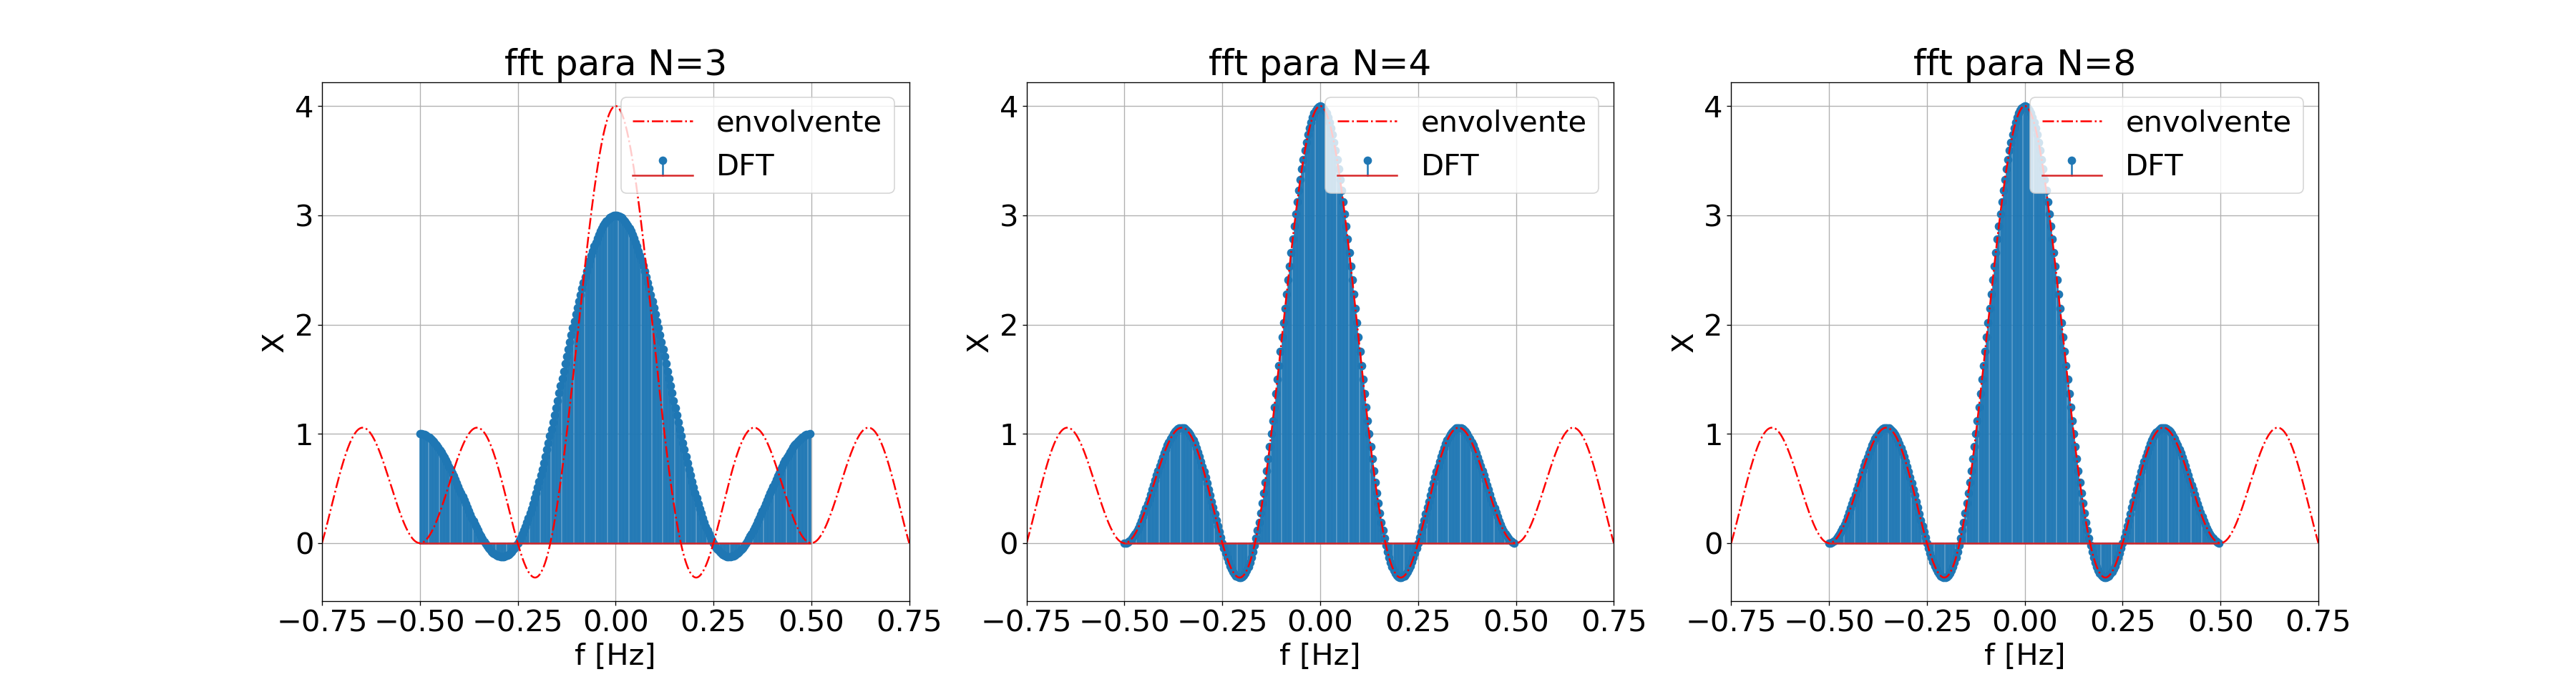
\includegraphics[width=\textwidth]{Img/punto_3_c.png}
\caption{\textit{fft} con zero-padding hasta 256 puntos para 3,4 y 8 puntos de la señal $x[n]$}
\label{fig.1c}
\end{figure}
Ahora es posible observar de mejor manera, lo comentado en el apartado anterior, como el zero-padding no agrega mas informacion al espectro sino que permite una mejor visualización del mismo, cuando se toman 3 puntos de la señal original, no se llega a tomar la señal completa si no que se recorta, por lo que el espectro si bien un aspecto similar, es mas ancho y de menor amplitud(al ser un cajon de 3 puntos y no de 4 puntos como la señal original), y para los casos de N=4 y N=8 que si se utiliza toda la informacion de la señal $x[n]$ se ve claramente que los valores de la DFT corresponden a muestras de la DTFT.
\end{document}